
%(BEGIN_QUESTION)
% Copyright 2006, Tony R. Kuphaldt, released under the Creative Commons Attribution License (v 1.0)
% This means you may do almost anything with this work of mine, so long as you give me proper credit

Are these two thermocouple circuits electrically equivalent?  That is, will they produce the same voltmeter indication given the same temperatures?  Why or why not?  The abbreviations are as follows: Fe = Iron, C = Constantan, Cu = Copper.

$$\includegraphics[width=15.5cm]{i00376x01.eps}$$

\underbar{file i00376}
%(END_QUESTION)





%(BEGIN_ANSWER)

The upper thermocouple circuit only has two junctions formed by dissimilar metals (the process junction, and the lower terminal block junction), and the lower thermocouple circuit has three, but they are equivalent circuits.  Imagine the voltmeter's copper wires shrinking in length until the two terminal block screws touch each other directly, and you will see that the same two Fe-C (Iron-Constantan) junctions exist in the same two circuits -- the voltmeter's copper wires are merely an intermediary step in a composite Fe-Cu-C junction, that behaves the same as an Fe-C junction (assuming both screw terminals are at the same temperature).

%(END_ANSWER)





%(BEGIN_NOTES)


%INDEX% Measurement, temperature: thermocouple

%(END_NOTES)


